\apendice{Documentación de usuario}

\section{Introducción}

En el último apéndice, indicaremos lo que necesitarán los usuarios de nuestra aplicación.

\section{Requisitos de usuarios}
 Enumeraremos los requisitos que se tienen que tener para poder usar la aplicación:
\begin{itemize}
 \item Si fuera la primera vez que vamos trabajar con está página, tendremos que descargarnos la base de datos y el código de la página del repositorio GitLab o GitHub.
 \item La extensión de metamask, en el navegador en el que despleguemos la pagina web.
 \item Conexión a Internet, ya que la página web el código cuenta con iconos que cogemos directamente de internet.
\end{itemize}
 
\section{Instalación}

Únicamente tendremos que descargar la extensión de metamask y la base de datos y código del repositorio GitLab \ref{intalacionE}.

\section{Manual del usuario}

Este manual va a constar la parte del administrador y usuario, el administrador podrá controlar a los usuarios y los usuarios podrán crear añadir nuevos productos y visualizar los productos que el mismo realizo. 

\subsection{Interfaz gráfica \textit{Front-End}\label{ref:front}}

En este apartado mostraremos el aspecto final de nuestra aplicación.

En este apartado explicaremos las diferentes pantallas de nuestra página web, y como consigue realizar la conexión con el método de pago mediante Metamask, y comprobar mediante la red Ethereum que el contrato se creó correctamente.

\paragraph{Inicio de sesión}\ref{fig:inicio}: la primera pantalla, nos resultará familiar de otras paginas web, hemos intentado que la página sea concisa, fácil e intuitiva. 

\begin{figure}[H]
    \centering
    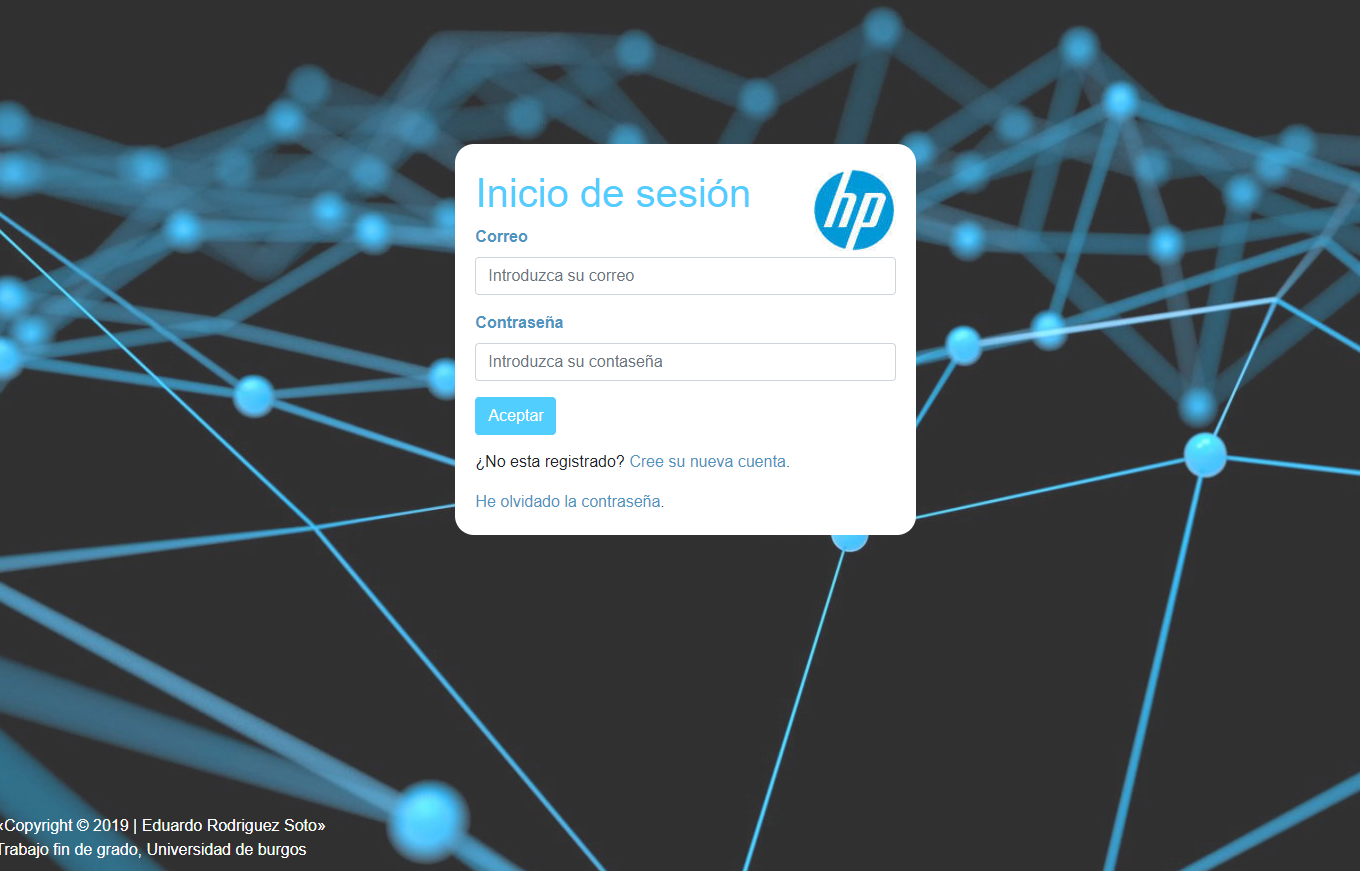
\includegraphics[width=\textwidth]{incioPag}
    \caption{Inicio de sesión}
    \label{fig:inicio}
\end{figure}

Tendremos que introducir el correo y la contraseña que previamente hayamos indicados a la hora de registrarnos y que tendremos en la misma página en un enlace ``¿No esta registrado? Cree su nueva cuenta''. En cualquier caso, si introducimos mal los datos, nos saltará mensaje de error y nos pedirá volver a iniciar sesión, teniendo la opción de poder enviarnos un correo de recordatorio de la contraseña al correo con el que nos registramos.

\paragraph{Crear nueva cuenta} \ref{fig:registro}: al igual que muchas páginas web, hemos creado la pantalla de registro (a esta página llegaremos desde la pantalla de inicio de sesión en la cual tendremos un apartado, ``¿No esta registrado? Cree su nueva cuenta''). Esta pantalla se compondrá de los campos: nombre, avatar, correo, contraseña, repetir contraseña y comprobación de que no eres un robot.

Todos los campos serán obligatorios, excepto el avatar, que en caso de no seleccionar ninguno, se le asignará el que tenemos por defecto.

\begin{figure}[h!]
    \centering
    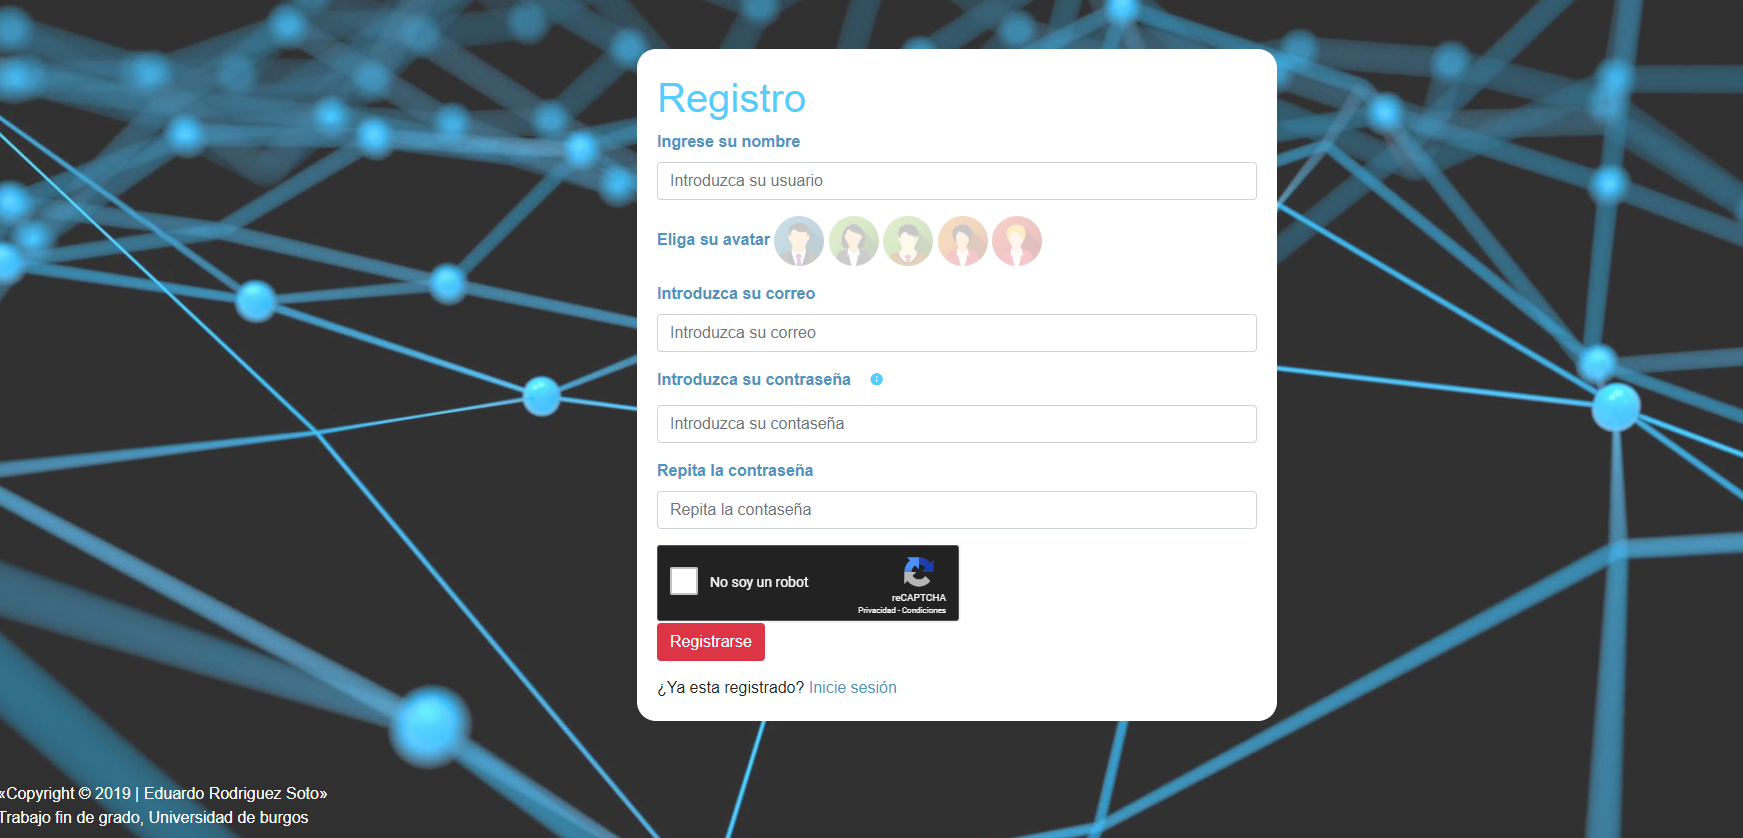
\includegraphics[width=\textwidth]{registro}
    \caption{Registrar nueva cuenta}
    \label{fig:registro}
\end{figure}

La contraseña tendrá que tener un formato típico (incluyendo mayúscula, minúscula y un número, y tendrá que ser compuesta de una cadena entre 8 y 12 elementos). En el caso de no introducir bien ambas contraseñas nos mostrará un error y nos llevará a la misma pantalla nuevamente, para volver a realizar el registro del usuario. En el caso de meter un correo ya existente a la hora de registrarse nos informará que ese correo ya está registrado. 

\paragraph{Olvido su contraseña} \ref{fig:olvido} suponemos que todo el mundo comete errores, y uno de los mas comunes es poder olvidar la contraseña, por ello hemos creado desde la pantalla de inicio de sesión, la opción de ``He olvidado la contraseña'', pinchando en en el enlace nos redirige a una página, la cual nos pedirá el correo del usuario, para así poder enviar un mensaje a su correo. Este nos dará una contraseña temporal para que el usuario pueda entrar en la cuenta y después modificar la contraseña, dependiendo si él quiere o no, en caso que el correo no esté en la base de datos, nos dará un mensaje de error de que ese usuario no está registrado\footnote{Esta página al trabajar en modo LocalHost, no estará habilitada, pero esta programada para funcionar cuando dispongamos de un dominio}.  s

\begin{figure}[H]
    \centering
    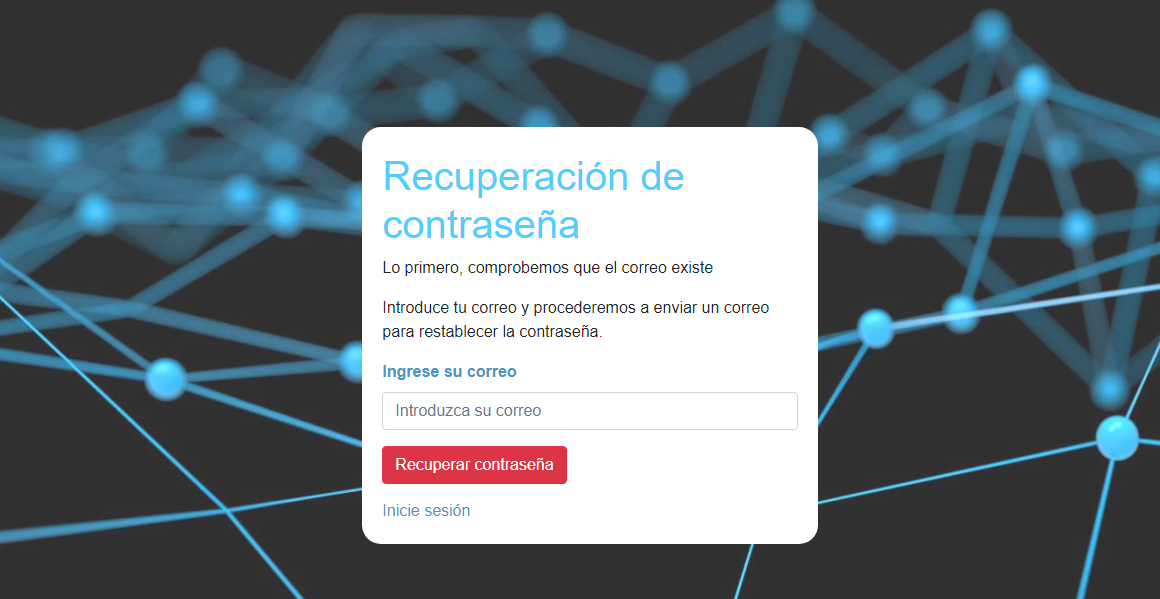
\includegraphics[width=\textwidth]{recuperarCnt}
    \caption{Recuperar contraseña}
    \label{fig:olvido}
\end{figure}

\paragraph{Página del administrador} \ref{fig:admin}: una vez reconocemos todos los enlaces de la pantalla de inicio, es hora de poder entrar en la sesión. Tendremos dos maneras de entrar: mediante el registro en la aplicación o por el uso de administrador, el cual será (admin/admin). Tendremos una pantalla como la siguiente: 

 \begin{figure}[H]
    \centering
    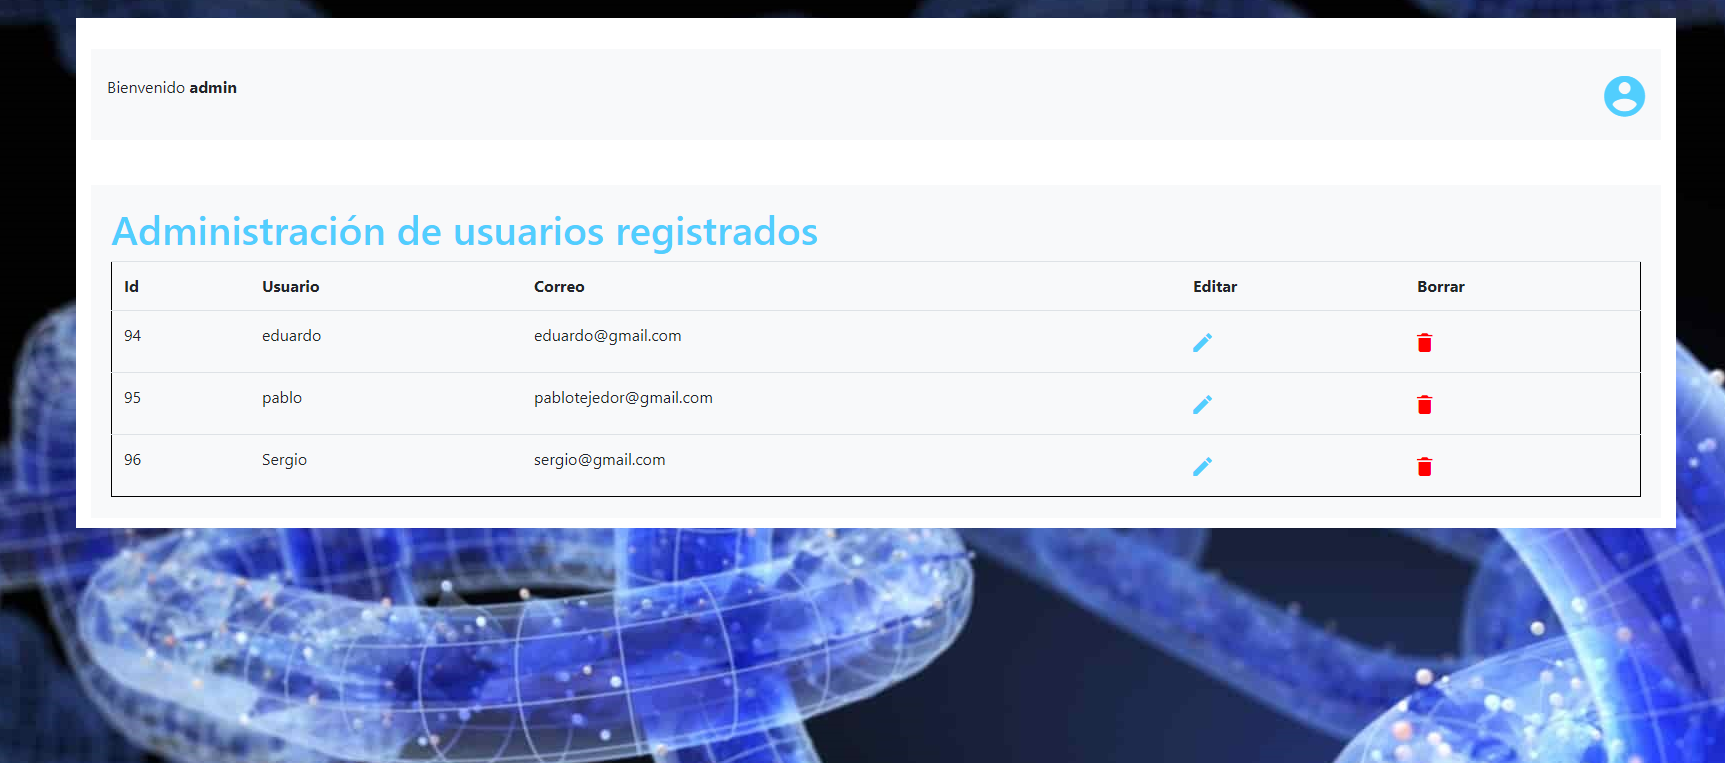
\includegraphics[width=\textwidth]{administrador}
    \caption{Administrador de usuarios}
    \label{fig:admin}
\end{figure}

El administrador será el responsable de poder gestionar y editar o borrar a los usuarios.

\paragraph{Administrador: \textit{Editar}} \ref{fig:editar}: en la cabecera nos informará mediante un mensaje de ``Bienvenido ...'' el usuario con el que se encuentra en cada momento. En la parte derecha tendremos un icono del avatar y en está pantalla nos permitirá cerrar sesión.

Si pulsamos en el lápiz azul de la columna editar de la fotografía \ref{fig:admin}  nos llevará a la siguiente pantalla:

 \begin{figure}[H]
    \centering
    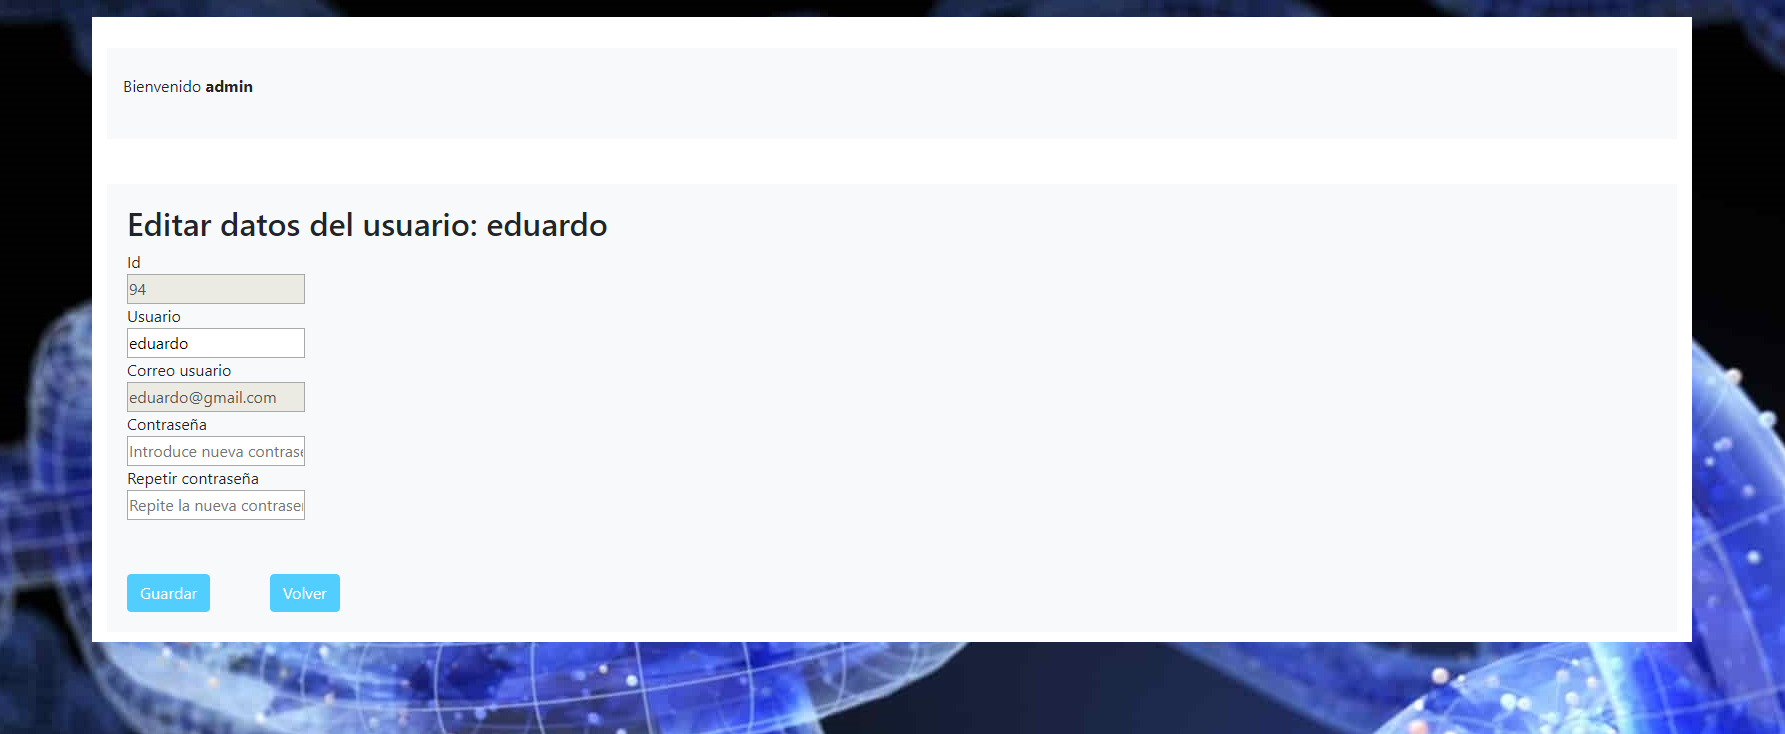
\includegraphics[width=\textwidth]{editarAdmin}
    \caption{Editar usuario desde administrador}
    \label{fig:editar}
\end{figure}

Nos mostrará los campos del usuario, pero únicamente podremos cambiar usuario y la contraseña, y nunca estos campos podrán quedar vacíos si hemos introducido algún valor anteriormente.

Cuando guardemos nos indicará si todo fue correcto, y, en caso de haber puesto las contraseñas incorrectas o el usuario vacío, nos mostrará un mensaje de error y tendremos que volver a realizar la misma operación, esta vez teniendo más cuidado y poniendo todo correctamente.

\paragraph{Administrador: \textit{Borrar}} \ref{fig:borrar}: así mismo, si queremos borrar tendremos que pulsar el icono de la papelera de la imágen \ref{fig:admin}, con esta acción nos mostrará un mensaje indicando si deseamos realizar la acción o no.

%\imagen{borrar2}{Borrar usuario desde administrador}
\begin{figure}[H]
	\centering
	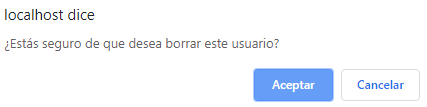
\includegraphics[width=0.7\textwidth]{confirmar}
	\caption{Mensaje confirmación}
	\label{fig:borrar}
\end{figure}

\paragraph{Opciones}\ref{fig:opciones}: una vez quedan explicadas las pantallas nos centramos en las que se involucran con el usuario de forma directa en su sesión.

Tendremos varias opciones en la pantalla de selección, los cuales explicaremos a continuación:
\begin{itemize}
	\item Añadir producto.
	\item Consultar el ultimo producto.
	\item Consultar todos los productos.
	\item Modificar datos (desde el avatar del usuario).
\end{itemize}

\begin{figure}[h!]
    \centering
    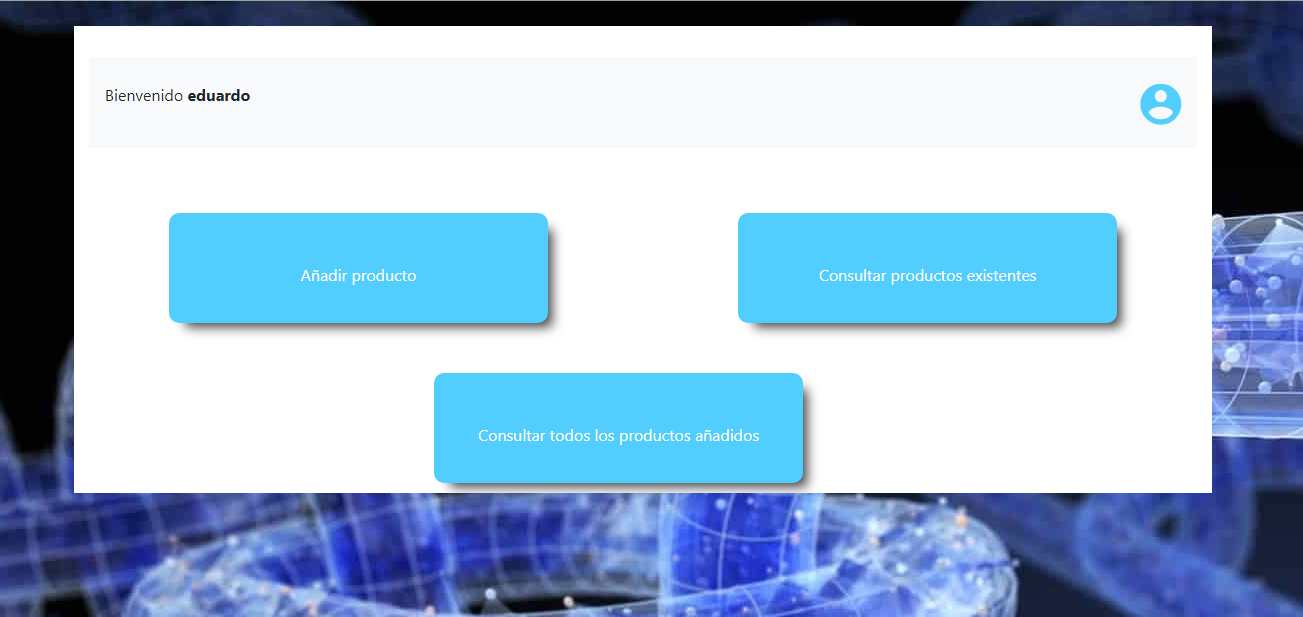
\includegraphics[width=0.7\textwidth]{opciones}
    \caption{Opciones a realizar por usuario}
    \label{fig:opciones}
\end{figure}

\paragraph{Añadir producto}: cuando pulsamos sobre la opción de añadir producto, esta automáticamente nos conectará con Metamask, pidiendo la contraseña \ref{fig:figura1e} (en caso de no estar logeados) o directamente nos dará la opción de conectar el proyecto con la cuenta que tengamos asociada de Metamask actualmente \ref{fig:figura2e}.

\begin{figure}[H]
	\begin{minipage}[b]{0.5\linewidth}
		\centering
		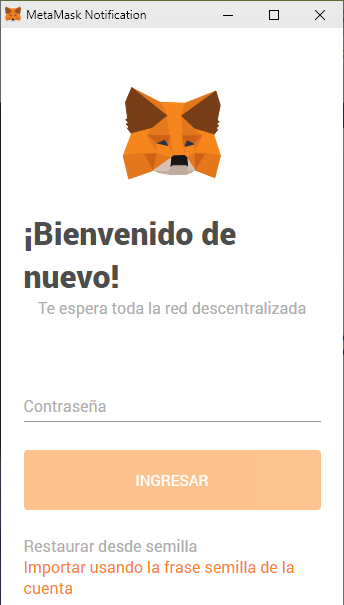
\includegraphics[width=\linewidth]{metamask-pantalla}
		\caption{Conexion Metamask}
		\label{fig:figura1e}
	\end{minipage}
	\hspace{0.5cm}
	\begin{minipage}[b]{0.5\linewidth}
		\centering
		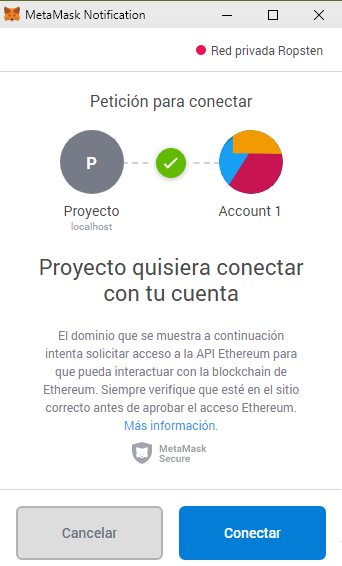
\includegraphics[width=\linewidth]{metamask-conexion}
		\caption{Conexion proyecto metamask}
		\label{fig:figura2e}
	\end{minipage}
\end{figure}

Una vez hemos completado el acceso y la conexión a metamask, tendremos que rellenar el producto que deseemos añadir \ref{fig:figura3e}, que serán los datos que almacenaremos en nuestro smart contract en la red Ethereum. 

\begin{figure}[H]
    \centering
    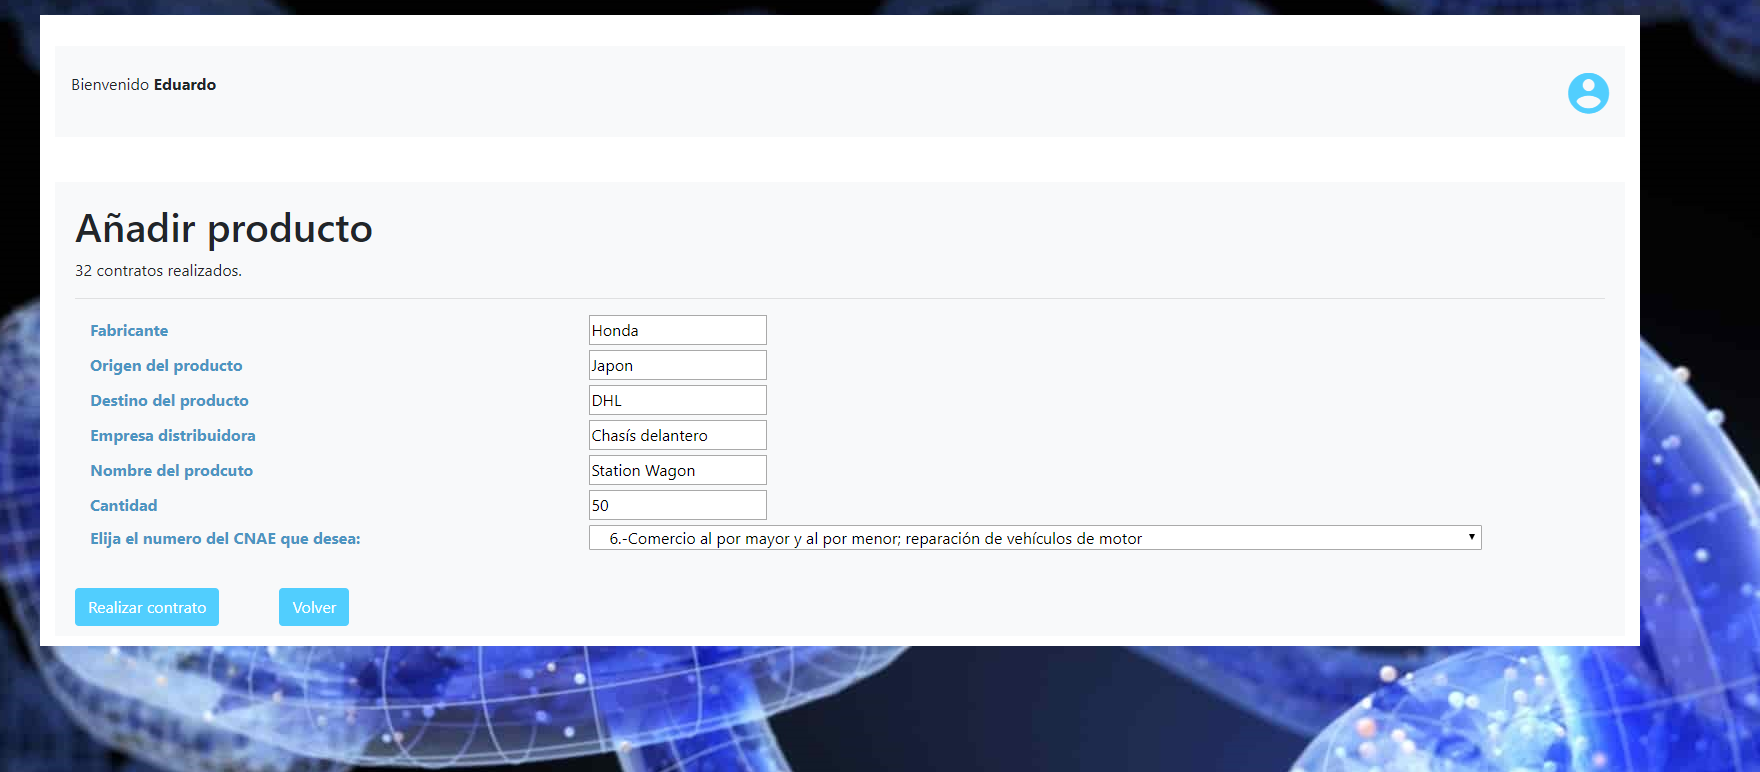
\includegraphics[width=1.00\textwidth]{anadirProdcuto1}
    \caption{Añadir producto}
    \label{fig:figura3e}
\end{figure}

Una vez rellenados los datos en nuestra pantalla, pulsaremos el botón de realizar contrato, esto nos mostrará nuevas pantallas que abrirá el conector de metamask para poder realizar el contrato \ref{fig:figura4e}, son las siguientes:

\begin{figure}[h!]
	\begin{minipage}[b]{0.5\linewidth}
		\centering
		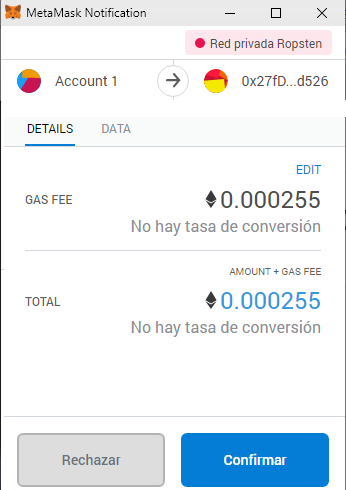
\includegraphics[width=\linewidth]{metamask-contrato}
		\caption{Confirmar el contrato}
		\label{fig:figura4e}
	\end{minipage}
\hspace{0.5cm}
	\begin{minipage}[b]{0.5\linewidth}
		\centering
		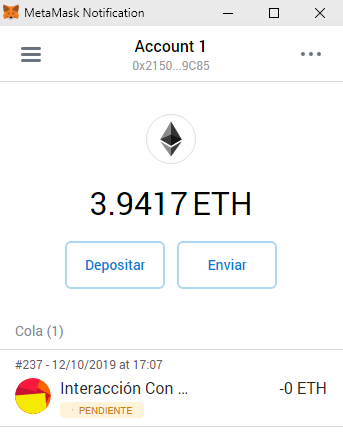
\includegraphics[width=\linewidth]{metamask-pendiente}
		\caption{Conexión pendiente}
		\label{fig:figura5e}
	\end{minipage}
	\begin{minipage}[b]{0.8\linewidth}
		\centering
		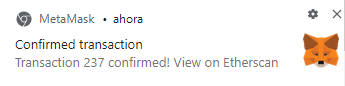
\includegraphics[width=\linewidth]{metamask-cofnirmado}
		\caption{Conexión confirmada}
		\label{fig:figura6e}
	\end{minipage}
\end{figure}

Cuando el usuario realiza la acción de añadir un nuevo producto, antes de guardar todos los datos, primero se tiene que conectar con la red Ethereum, y hasta que no se crea el \textit{smart contract}, estos datos no quedarán debidamente guardados en la base de datos. 
 
Una vez que se haya confirmado la transacción \ref{fig:figura6e} en metamask, los datos se habrán guardado tanto en nuestra base de datos como en la red Ethereum de la red privada Ropsten. Si por un causal hubiera fallo de red o no tuviéramos conexión a la red, estos datos se perderían y tendríamos que realizar el contrato nuevamente para guardarlos. 

Para poder ver dicha transacción existen dos opciones: en la red Ethereum o bien mediante la nuestra página web.

En la red tendremos varias formas de llegar, pulsando directamente cuando nos sale el aviso de la \ref{fig:figura6e}, también se puede llegar pulsando en el icono de Metamask y la transacción que deseemos pulsar sobre la fecha ver en Etherscan. Una vez pulsado nos redirige a una pagina, llamada rospten.etherscan.io y el código de la transacción según cuál sea la que estamos trabajando.

En esta nueva pagina podremos ver toda la información del contrato mediante dos pestañas encontradas en la parte superior de la página:\hfill

\begin{itemize}
 \item  \textbf{Overview} \ref{fig:figura7e}: el estado y la hora de la transacción, la cuenta desde la que se hizo y a la cuenta que se realiza la transacción, el gas y el coste de ether. 
 
 \item \textbf{Event Logs} \ref{fig:figura8e}: en la cual podremos ver los datos que hemos introducido en nuestra pantalla de añadir producto(al principio nos saldrán todas los datos en formato hexadécimal y convertirlo a formato text o formato numérico según el datos que estemos buscando).
 \end{itemize}
 \begin{figure}[H]
    \centering
    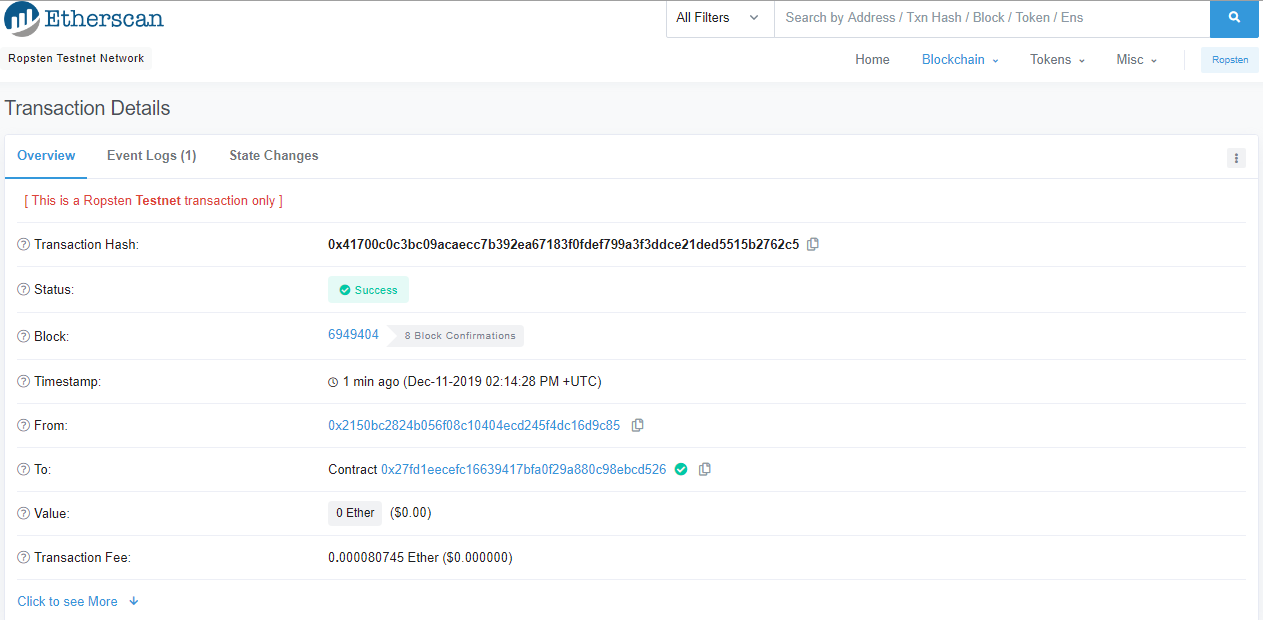
\includegraphics[width=\textwidth]{etherscan}
    \caption{Información del contrato creado vistos por Etherscan}
    \label{fig:figura7e}
\end{figure}
\begin{figure}[H]
    \centering
    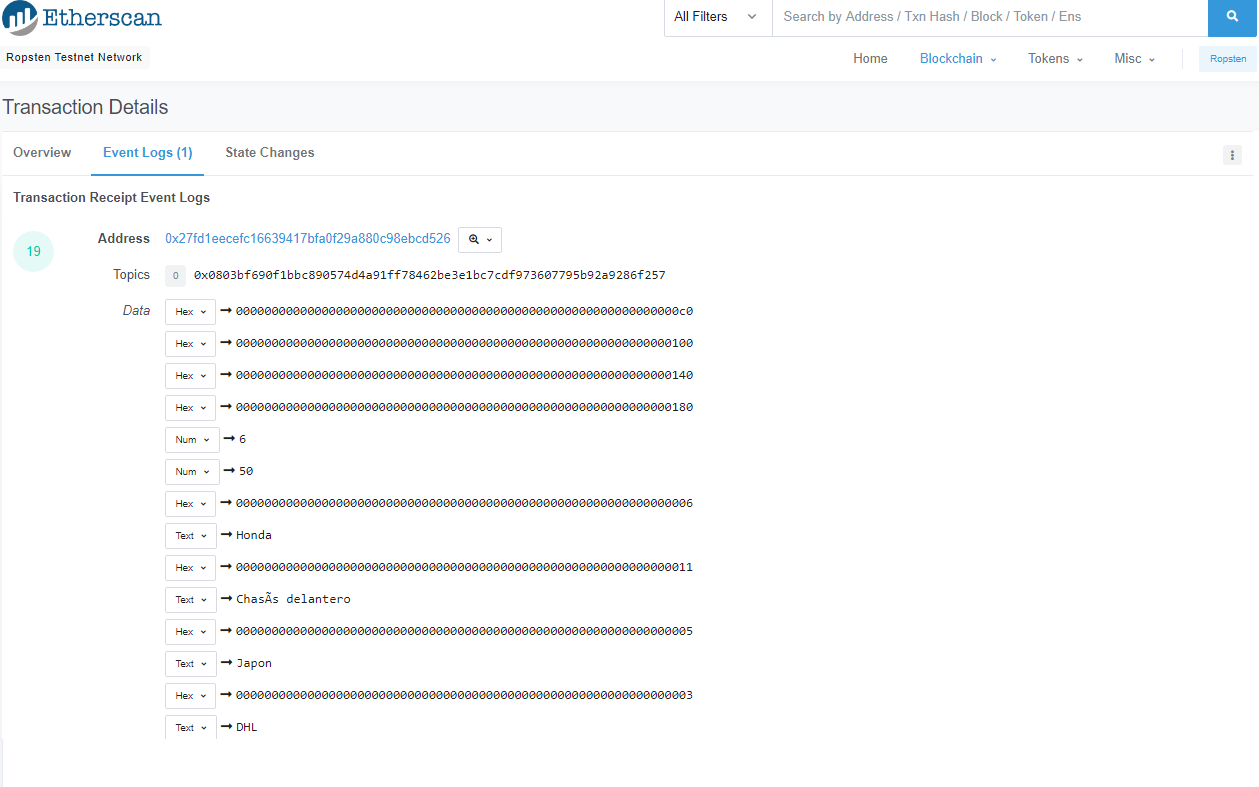
\includegraphics[width=\textwidth]{datos-etherscan}
    \caption{Datos proporcionados por Etherscan}
    \label{fig:figura8e}
\end{figure}


Una vez vistos todos estos datos en cuanto a la conexión de la red con Metamask y, esta a su vez, con la red Ropsten y Etherscan, ya tendríamos nuestro contrato ubicado en la red en todo momento, siempre que tengamos el enlace o bien la aplicación de metamask en la transacción que deseemos saber los datos.

\paragraph{Consultar todas las transacciones y la última transacción} \ref{fig:figura9e}: en el apartado anterior se explicó como observar la transacción que se realizó en un momento dado gracias a la red Etherscan. La otra forma de poder observarlas es dar a ``volver'', una vez confirmada la transacción. Lo que intentamos realizar con la creación de estos dos botones es que el usuario de la página no tenga que perder el tiempo entrando en esta red y poder buscarlo de forma más eficaz.

\begin{figure}[h!]
	\centering
	\begin{minipage}{0.8\linewidth}
		\centering
    	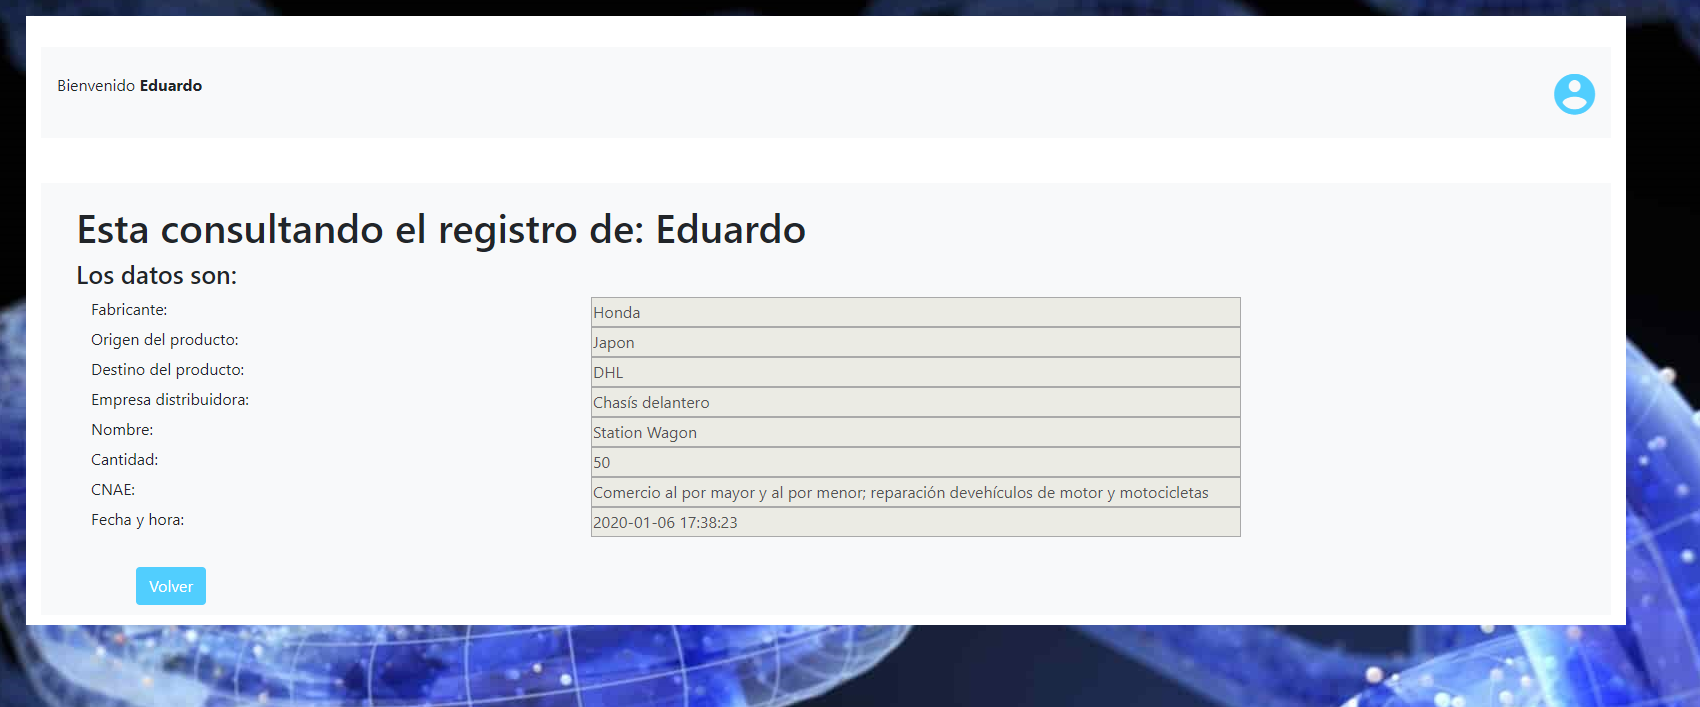
\includegraphics[width=\textwidth]{ultimoContrato}
    	\caption{Visualización del último producto}
    	\label{fig:figura9e}
	\end{minipage}
	\begin{minipage}{0.8\linewidth}
		 \centering
    	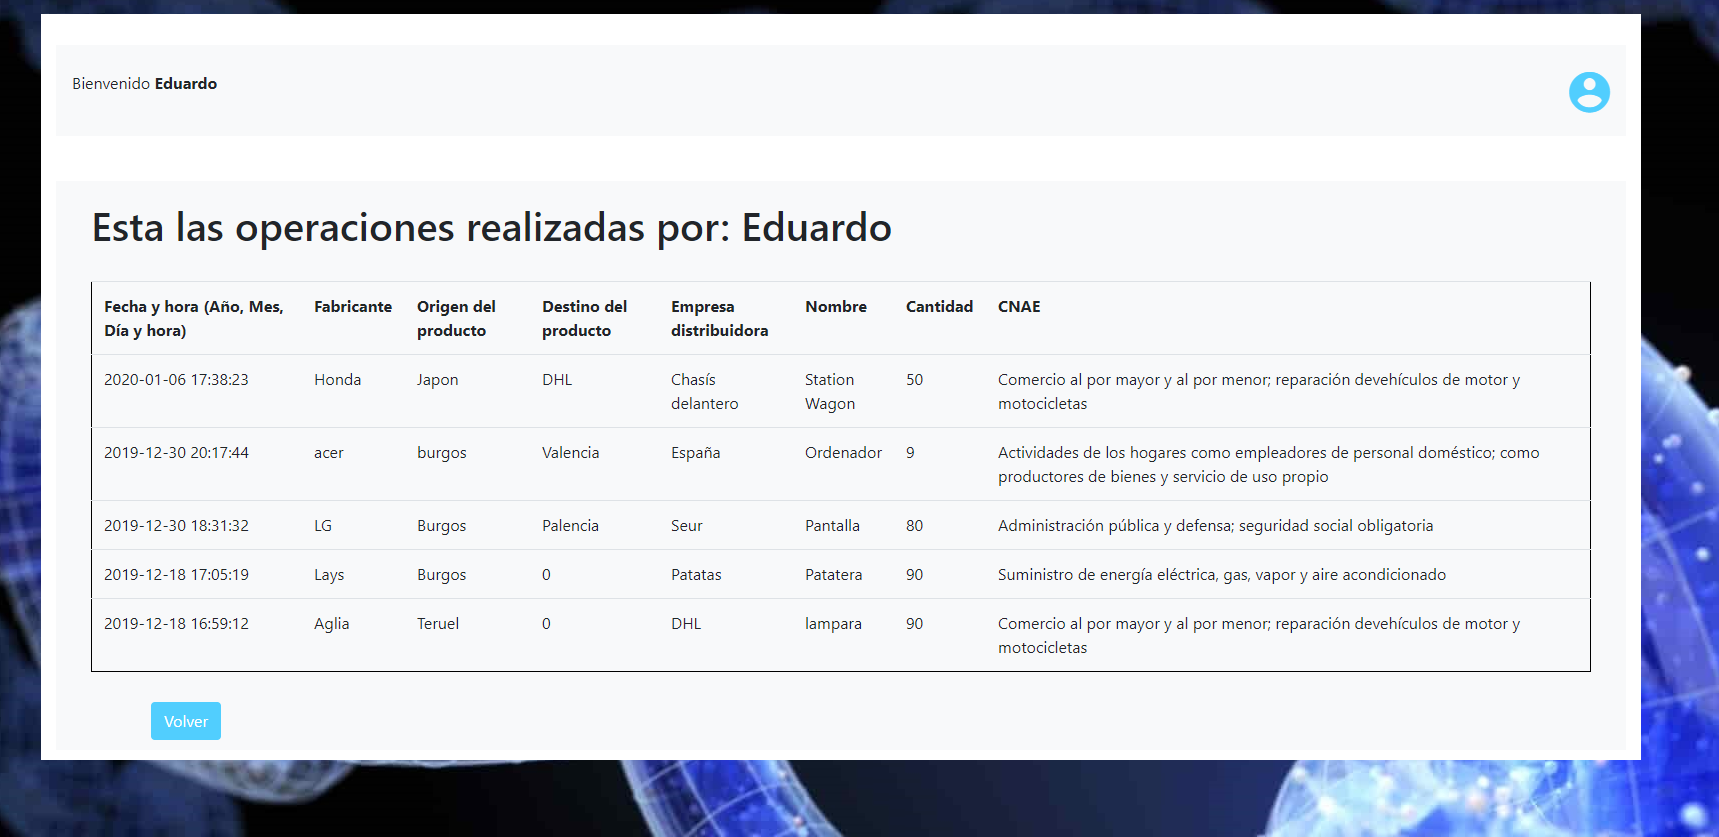
\includegraphics[width=\textwidth]{todosContratos}
    	\caption{Visualización de todos los productos realizados}
    	\label{fig:figura10e}
	\end{minipage}
\end{figure}

Las transacciones que realicemos nunca se podrán modificar ni borrar. Cierto es que en nuestra página (hemos decidido que mientras el usuario tenga una cuenta. Exista la transacción, pero si borramos al usuario, estaremos eliminado todos los contratos que creó de nuestra base de datos) pero en la red de Etherscan se podrán seguir visualizando de forma permanente, tal y como se explicó anteriormente. 
